\documentclass[a4paper,12pt]{article}     %页面大小和字体大小
\usepackage{ctex}
\usepackage{geometry}
\usepackage{mathptmx}
\usepackage{amsmath}
\usepackage{graphicx}
\usepackage[T1]{fontenc}
\geometry{left=2.0cm, right=2.0cm, top=3.0cm, bottom=3.0cm}   %页边距
\linespread{1.5}      %行距

\begin{document}

\begin{center}   %居中设置
孟澍 \ 3210101819
\end{center}

\noindent %顶格(不缩进)
\textbf{3.38}\\
A memory address is a uniquely identifiable memory location. Memory's addressability is the number of bits stored in each memory location.

~\\
\textbf{3.40}\\
a. \ The address space is 4 because the memory is addressed by 2 bits.\\
b. \ The addressability is 4 because 4 bits is stored in each memory location.\\
c. \ 0001.\\

~\\
\textbf{3.53}\\
~\\
\begin{tabular}{c|c|c|c|c|c|c|c|c|}
  \hline
  & cycle0 & cycle1 & cycle2 & cycle3 & cycle4 & cycle5 & cycle6 & cycle7 \\
  \hline
  D2 & 0 & 1 & 1 & 1 & 1 & 0 & 0 & 0 \\
  \hline
  D1 & 0 & 1 & 1 & 0 & 0 & 1 & 1 & 0 \\
  \hline
  D0 & 0 & 1 & 0 & 1 & 0 & 1 & 0 & 1 \\
  \hline
\end{tabular}
\\
~\\
It prolongs the cycle of the clock.

\newpage
\textbf{3.61}\\
~\\
a. \
\begin{tabular}{|c|c|c||c|c|c|}
  \hline
  S1 & S0 & X & Z & S1' & S0' \\
  \hline
  \hline
  0 & 0 & 0 & 1 & 0 & 0 \\
  \hline
  0 & 0 & 1 & 1 & 0 & 1 \\
  \hline
  0 & 1 & 0 & 0 & 1 & 0 \\
  \hline
  0 & 1 & 1 & 0 & 0 & 0 \\
  \hline
  1 & 0 & 0 & 0 & 0 & 1 \\
  \hline
  1 & 0 & 1 & 0 & 1 & 0 \\
  \hline
  1 & 1 & 0 & 0 & 0 & 0 \\
  \hline
  1 & 1 & 1 & 0 & 0 & 0 \\
  \hline
\end{tabular}\\
~\\
b. \ \begin{figure}[h] 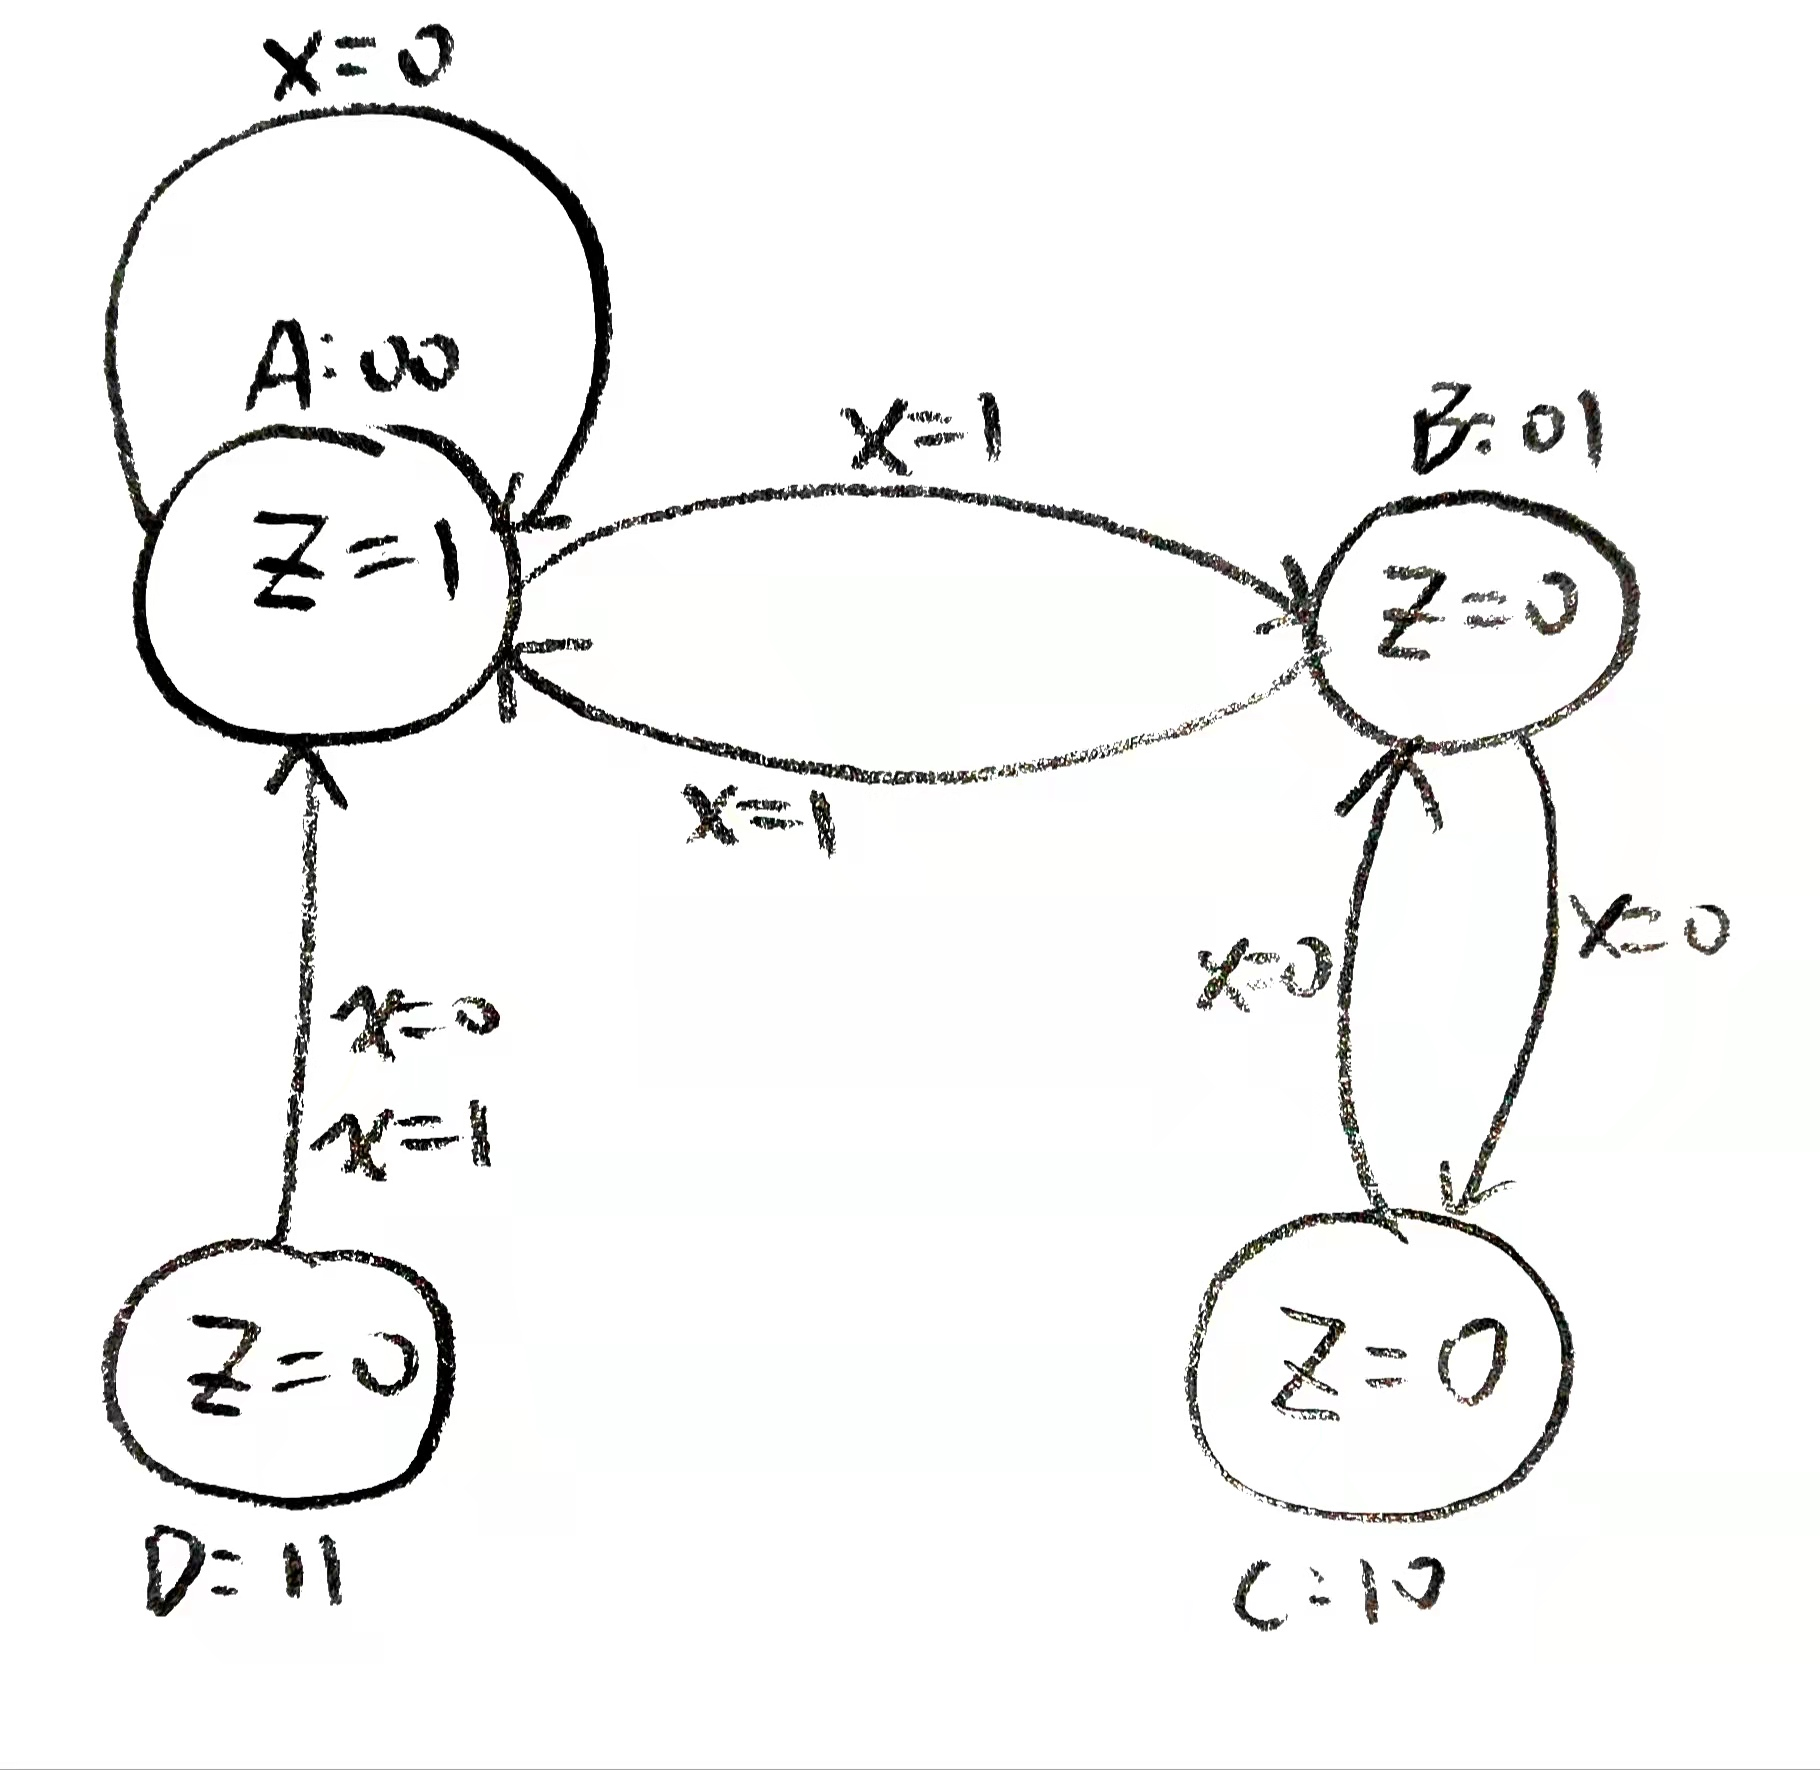
\includegraphics[width = 0.5\textwidth]{../fig/3.61.jpeg} \end{figure}

\newpage
\noindent %顶格(不缩进)
\textbf{4.1}\\
Memory: store the computer program.\\
A processing unit: process information. Do arithmetical and logical oprations.\\
Input: send information into the computer.\\
Output: provide or display the result of the program's execution.\\
A control unit: keep track of which both where we are within the process of executing the program and where we are in the process of executing each instruction.\\


~\\
\textbf{4.7}\\
6 bits are needed to represent the opcode. 5 bits are needed to represent each register. Consequently, there are 16 bits remained for IMM. The range of values can be represented by IMM is $-2^{15} \mbox{\textasciitilde} 2^{15}-1.$



\end{document}
